\PassOptionsToPackage{unicode=true}{hyperref} % options for packages loaded elsewhere
\PassOptionsToPackage{hyphens}{url}
\documentclass[12pt,ignorenonframetext,aspectratio=169]{beamer}
\IfFileExists{pgfpages.sty}{\usepackage{pgfpages}}{}
\setbeamertemplate{caption}[numbered]
\setbeamertemplate{caption label separator}{: }
\setbeamercolor{caption name}{fg=normal text.fg}
\beamertemplatenavigationsymbolsempty
\usepackage{lmodern}
\usepackage{amssymb}
\usepackage{amsmath}
\usepackage{ifxetex,ifluatex}
\usepackage{fixltx2e} % provides \textsubscript
\ifnum 0\ifxetex 1\fi\ifluatex 1\fi=0 % if pdftex
  \usepackage[T1]{fontenc}
  \usepackage[utf8]{inputenc}
\else % if luatex or xelatex
  \ifxetex
    \usepackage{mathspec}
  \else
    \usepackage{fontspec}
\fi
\defaultfontfeatures{Ligatures=TeX,Scale=MatchLowercase}






%
\fi

  \usetheme[]{iqss}






% use upquote if available, for straight quotes in verbatim environments
\IfFileExists{upquote.sty}{\usepackage{upquote}}{}
% use microtype if available
\IfFileExists{microtype.sty}{%
  \usepackage{microtype}
  \UseMicrotypeSet[protrusion]{basicmath} % disable protrusion for tt fonts
}{}


\newif\ifbibliography


\hypersetup{
      pdftitle={Production relationships},
        pdfauthor={Deependra Dhakal},
          pdfborder={0 0 0},
    breaklinks=true}
%\urlstyle{same}  % Use monospace font for urls







% Prevent slide breaks in the middle of a paragraph:
\widowpenalties 1 10000
\raggedbottom

  \AtBeginPart{
    \let\insertpartnumber\relax
    \let\partname\relax
    \frame{\partpage}
  }
  \AtBeginSection{
    \ifbibliography
    \else
      \let\insertsectionnumber\relax
      \let\sectionname\relax
      \frame{\sectionpage}
    \fi
  }
  \AtBeginSubsection{
    \let\insertsubsectionnumber\relax
    \let\subsectionname\relax
    \frame{\subsectionpage}
  }



\setlength{\parindent}{0pt}
\setlength{\parskip}{6pt plus 2pt minus 1pt}
\setlength{\emergencystretch}{3em}  % prevent overfull lines
\providecommand{\tightlist}{%
  \setlength{\itemsep}{0pt}\setlength{\parskip}{0pt}}

  \setcounter{secnumdepth}{0}


  \usepackage{booktabs}
  \usepackage{longtable}
  \usepackage{emptypage}
  \usepackage{array}
  \usepackage{multirow}
  \usepackage{wrapfig}
  \usepackage{float}
  \usepackage{colortbl}
  \usepackage{pdflscape}
  \usepackage{tabu}
  \usepackage{threeparttable}
  \usepackage{threeparttablex}
  \usepackage[normalem]{ulem}
  \usepackage{rotating}
  \usepackage{makecell}
  \usepackage{xcolor}
  \usepackage{tikz} % required for image opacity change
  \usepackage[absolute,overlay]{textpos} % for text formatting
  \usepackage[utf8]{inputenc}
  \usetikzlibrary{mindmap}

  % this font option is amenable for beamer
  \setbeamerfont{caption}{size=\tiny}


%% IQSS overrides
\iqsssectiontitle{Outline}

\AtBeginSection[]{
  \title{\insertsectionhead}
  {
    \definecolor{white}{rgb}{0.776,0.357,0.157}
    \definecolor{iqss@orange}{rgb}{1,1,1}
    \ifnum \insertmainframenumber > \insertframenumber
    \frame{
      \frametitle{\iqsssectiontitleheader}
      \tableofcontents[currentsection]
    }
    \else
    \frame{
      \frametitle{Backup Slides}
      \tableofcontents[sectionstyle=shaded/shaded,subsectionstyle=shaded/shaded/shaded]
    }
    \fi
  }
}

\AtBeginSubsection[]{}

%%


  \title[]{Production relationships}



  \author[
        Deependra Dhakal
    ]{Deependra Dhakal}

  \institute[
    ]{
    GAASC, Baitadi \and Tribhuwan University
    }

\date[
      \today
  ]{
      \today
        }

\begin{document}

% Hide progress bar and footline on titlepage
  \begin{frame}[plain]
  \titlepage
  \end{frame}



\hypertarget{production-relationships}{%
\section{Production relationships}\label{production-relationships}}

\begin{frame}{}
\protect\hypertarget{section}{}
\begin{itemize}
\tightlist
\item
  All major production relationships can be categorized under three
  categories. i.e.:

  \begin{enumerate}
  \tightlist
  \item
    Factor-product relationship
  \item
    Factor-factor relationship
  \item
    Product-product relationship
  \end{enumerate}
\end{itemize}
\end{frame}

\hypertarget{cost-concepts}{%
\section{Cost concepts}\label{cost-concepts}}

\begin{frame}{Background}
\protect\hypertarget{background}{}
\begin{itemize}
\tightlist
\item
  A farmer can increase his income by one of two ways:

  \begin{enumerate}
  \tightlist
  \item
    Increasing the production
  \item
    Reducing the cost of production
  \end{enumerate}
\end{itemize}
\end{frame}

\begin{frame}{Cash cost and non-cash cost}
\protect\hypertarget{cash-cost-and-non-cash-cost}{}
\begin{itemize}
\tightlist
\item
  In economics cost means the total efforts involved in the production
  of a commodity while expense of production only signify money costs.
\item
  Cash costs are incurred when resources are purchased and used
  immediately in the production process.
\item
  Non-cash cost consist of depreciation and payments to resources owned
  by the farmers e.g., depreciation on tractor, equipment, buildings,
  payment made to the farmer himself or family labor, management and
  owned capital.
\end{itemize}
\end{frame}

\begin{frame}{Total cost}
\protect\hypertarget{total-cost}{}
\begin{itemize}
\tightlist
\item
  Fixed costs plus variable costs equal total costs. Total costs are
  required for computing net revenue. Net revenue is equal to total
  revenue less total cost.
\item
  Whether a particular cost item will be considered as fixed or variable
  one depends upon whether the input concerned is fixed or variable for
  the problem under consideration.
\item
  During long run planning period all inputs are variable. Thus in long
  run there are no fixed costs.
\item
  Total cost = Fixed cost + Variable cost
\end{itemize}
\end{frame}

\begin{frame}{Marginal cost}
\protect\hypertarget{marginal-cost}{}
\begin{itemize}
\tightlist
\item
  The additional cost of doing a little bit more (or 1 unit more if a
  unit can be measured) of an activity.
\item
  How do you make a rational decision about when the alarm should go
  off? What you have to do is to weigh up the costs and benefits of
  additional sleep. Each extra minute in bed gives you more sleep (the
  marginal benefit), but gives you more of a rush when you get up (the
  marginal cost).
\item
  The decision is therefore based on the costs and benefits of extra
  sleep, not on the total costs and benefits of a whole night's sleep.
\end{itemize}
\end{frame}

\begin{frame}{Opportunity cost}
\protect\hypertarget{opportunity-cost}{}
\begin{itemize}
\tightlist
\item
  The farm resources have alternative uses.
\item
  The price that will be required to prevent the transference of factors
  to other uses is called ``opportunity cost'' or ``alternative cost''.
\item
  The price which should be put on any input is therefore the return
  which must be given up in the next best alternative use.
\item
  Thus every resource used in production has one true cost: opportunity
  cost.
\item
  Suppose a farmer has 40 kgs of fertilizer; it adds Rs 250 to the total
  revenue from wheat and Rs 200 to the revenue from barley. If he
  fertilizes barley, his opportunity cost is Rs 250, which he has
  foregone on wheat. If he fertilizes wheat, his opportunity cost is Rs
  200, foregone on barley.
\end{itemize}
\end{frame}

\begin{frame}{}
\protect\hypertarget{section-1}{}
\begin{itemize}
\tightlist
\item
  Thus once purchased, market price of input becomes irrelevant to the
  problem of its allocation among alternative uses.
\item
  In case of durable resources such as machinery or land which are used
  in production, the opportunity cost is defined to be the amount that
  total capital investment could earn if invested in its best
  alternative use.
\item
  For simplest case, the opportunity cost will be interest that a
  deposit of money in a bank would fetch.
\end{itemize}
\end{frame}

\begin{frame}{Return concepts}
\protect\hypertarget{return-concepts}{}
\begin{itemize}
\tightlist
\item
  Gross return = Total production \(\times\) price
\item
  Net return = Gross return - Total cost
\item
  Returns to fixed farm resources(or returns over variable costs) =
  Gross returns - Variable cost
\end{itemize}
\end{frame}

\begin{frame}{Rational decision}
\protect\hypertarget{rational-decision}{}
\begin{itemize}
\tightlist
\item
  Doing more of an activity if its marginal benefit exceeds its marginal
  cost and doing less if its marginal cost exceeds its marginal benefit.
\item
  Rational decisions are made with rational choices; that involve
  weighing up the benefit of any activity against its opportunity cost.
\end{itemize}
\end{frame}

\hypertarget{product}{%
\section{Product}\label{product}}

\begin{frame}{Total product (TP)}
\protect\hypertarget{total-product-tp}{}
\begin{itemize}
\tightlist
\item
  A given level of total product is always associated with a particular
  level of input(s) use with a given technology.
\item
  The total volume or amount of final output produced by a firm using
  given inputs in a given period of time is called \textbf{Total
  product}.
\item
  Production function is often presented as total output curve because
  total product curve and production function curve are closely
  associated.
\end{itemize}
\end{frame}

\begin{frame}{Average product (AP)}
\protect\hypertarget{average-product-ap}{}
\begin{itemize}
\tightlist
\item
  The term average product refers to the average productivity of
  resources. It is the ratio of total product (TP) to the quantity of
  input used in producing that amount of product, i.e., at any point on
  production function, it is the total output divided by the total input
  used.
\end{itemize}

\[
AP = \frac{Y}{X}
\]

Where Y is product and X the input(s).
\end{frame}

\begin{frame}{Marginal product}
\protect\hypertarget{marginal-product}{}
\begin{itemize}
\tightlist
\item
  The term marginal product refers to the quantity which additional
  (marginal) unit of factor-input adds to the total product. The
  marginal product (MP) at any level of the variable input can be
  approximated by dividing the addition to total output by the addition
  to total input:
\end{itemize}

\[
MP = \frac{\Delta Y}{\Delta X}
\]

Here, \(\Delta\) refers to the change in or addition to the product or
the input.

\begin{itemize}
\tightlist
\item
  It is the rate of change in total product at a given point as the
  quantity of input changes.
\item
  Although, average productivity provides some guidelines as to the
  manner in which resources are allocated, it is marginal productivity
  which provides the final criterion in determining optimum use of
  limited resources.
\end{itemize}
\end{frame}

\begin{frame}{Average marginal product}
\protect\hypertarget{average-marginal-product}{}
\begin{itemize}
\tightlist
\item
  The average marginal product indicates the productivity values between
  the two relevant input levels.
\end{itemize}

\begin{table}

\caption{\label{tab:marginal-product1}Example 1}
\centering
\fontsize{6}{8}\selectfont
\begin{tabular}[t]{rr}
\toprule
input & output\\
\midrule
0 & 10\\
5 & 20\\
10 & 30\\
15 & 40\\
\bottomrule
\end{tabular}
\end{table}

\begin{table}

\caption{\label{tab:marginal-product2}Example 2}
\centering
\fontsize{6}{8}\selectfont
\begin{tabular}[t]{rr}
\toprule
input & output\\
\midrule
0 & 10\\
5 & 30\\
10 & 45\\
15 & 50\\
\bottomrule
\end{tabular}
\end{table}
\end{frame}

\begin{frame}{}
\protect\hypertarget{section-2}{}
\begin{itemize}
\tightlist
\item
  In Example 1 (Table \ref{tab:marginal-product1}), when
  \(\Delta X = 5\), \(\Delta Y = 10\), then
  \(\frac{\Delta Y}{\Delta X} = \frac{10}{5} = 2.0\)
\item
  In Example 2 (Table \ref{tab:marginal-product2}), when
  \(\Delta X = 5\), \(\Delta Y = 20\) for first unit of input, 15 for
  second and 5 for third addition of input. It indicates that with each
  unit change in X from 0 to first addition of inputs, there is a change
  in 2 units of Y (\(\frac{\Delta Y}{\Delta X} = \frac{20}{5} = 4.0\)).
  The Marginal product of variable unit can be thus approximated by
  dividing addition to total output by addition to total input. The
  marginal product, however, has decreased upon further addition of
  inputs to the first input level. i.e., when the input level is 15 (0 +
  5 + 10), the additional 5 (10-5) unit input have given rise to only 15
  (45-30) unit of output, hence the marginal product
  (\(\frac{\Delta Y}{\Delta X} = \frac{15}{5} = 3.0\)). This is
  reduction from the previous value of MP of 4.
\end{itemize}
\end{frame}

\begin{frame}{Example: Production function of wheat}
\protect\hypertarget{example-production-function-of-wheat}{}
To isolate the relationship between nitrogen and wheat yields, the
agronomists (or other biophysical scientists) will hold constant all
inputs other than the one that they are isolating, in this case
nitrogen.

\[Y = f(N | L, K, M, A)\]

This relationship is highly important, since too little nitrogen means
the yields will be lower than the potential, and too much nitrogen will
``burn'' the crop, causing smaller yields. Figure
\ref{fig:nitrogen-wheat} shows the connection between nitrogen
applications and wheat yields.
\end{frame}

\begin{frame}{}
\protect\hypertarget{section-3}{}
\begin{figure}
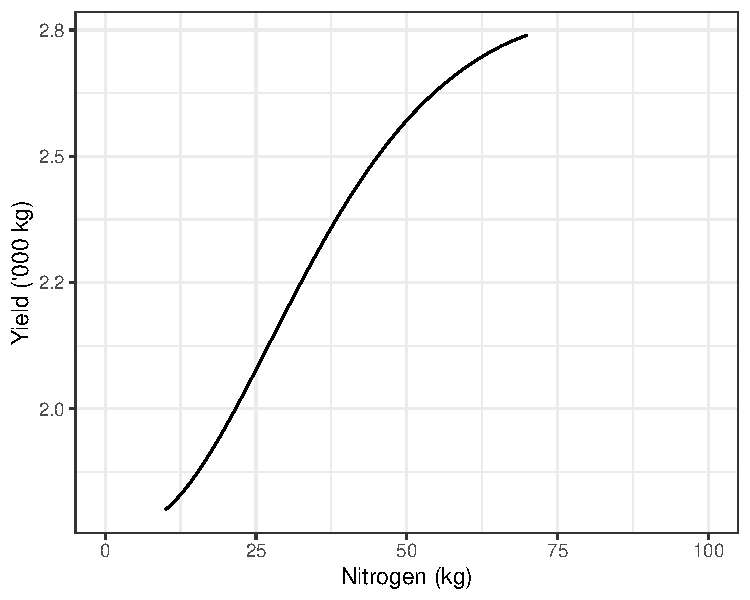
\includegraphics[width=0.5\linewidth]{03-production_relationship_files/figure-beamer/nitrogen-wheat-1} \caption{Relationship between nitrogen application and yield}\label{fig:nitrogen-wheat}
\end{figure}
\end{frame}

\begin{frame}{}
\protect\hypertarget{section-4}{}
\begin{figure}
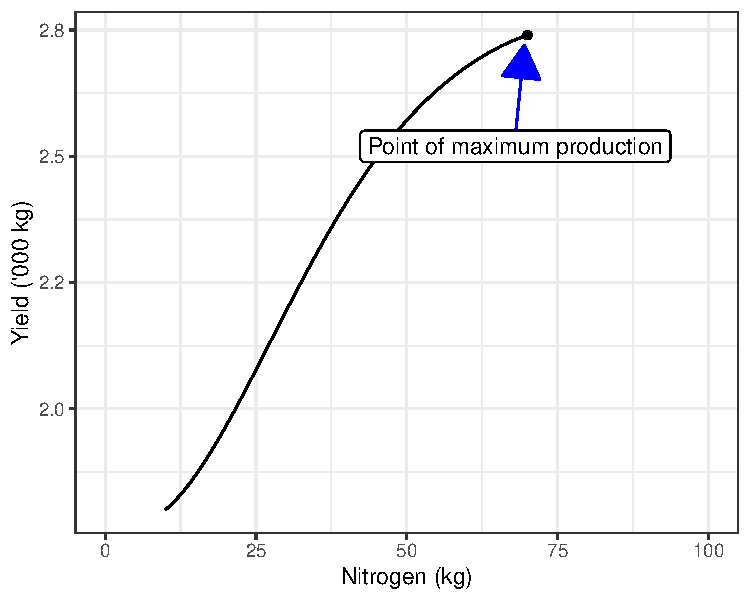
\includegraphics[width=0.5\linewidth]{03-production_relationship_files/figure-beamer/nitrogen-wheat-optimum-production-1} \caption{Relationship between nitrogen application and yield}\label{fig:nitrogen-wheat-optimum-production}
\end{figure}
\end{frame}

\begin{frame}{Concept of optimum production}
\protect\hypertarget{concept-of-optimum-production}{}
\begin{itemize}
\tightlist
\item
  The point of maximum physical wheat yield (N*) is not always the
  optimal economic wheat yield. This is because nitrogen is a scarce
  resource, and costs money to purchase. In fact, fertilizer is one of
  the major costs of production for farmers in most agricultural
  regions.
\item
  If nitrogen were free, then the optimal application to a wheat field
  would always be N* in Figure \ref{fig:nitrogen-wheat}, since this is
  the level of nitrogen that maximizes production.
\item
  However, since it costs money to purchase and use fertilizer, the
  farmer will stop applying it at a point to the left of N*. Finding the
  optimal amount of nitrogen to apply requires application of economic
  principles. Economic reasoning will help determine the exact point
  where the benefits of using N minus the costs are maximized.
\item
  Producers will not maximize production, because it costs too much.
  Instead, they will maximize profits.
\end{itemize}
\end{frame}

\hypertarget{bibliography}{%
\section{Bibliography}\label{bibliography}}

\begin{frame}{For more information}
\protect\hypertarget{for-more-information}{}
\end{frame}




\end{document}
